% =============================================================================
% GRPO-REGISTRY: A Living Catalog of Stack Fields and Variant Deltas
% =============================================================================
% Pillar 1 of the ZVF Program. Companion paper to MIN-REPORT-RL (position).
%
% This standalone article-class draft uses the program's canonical shared
% bibliography at platform_hybrid/paper/references.bib.
% =============================================================================

\documentclass[11pt]{article}

\usepackage[utf8]{inputenc}
\usepackage[T1]{fontenc}
\usepackage[margin=1in]{geometry}
\usepackage{hyperref}
\usepackage{url}
\usepackage{booktabs}
\usepackage{amsmath}
\usepackage{amssymb}
\usepackage{xcolor}
\usepackage{enumitem}
\usepackage{microtype}
\usepackage{graphicx}
\usepackage{longtable}
\usepackage{listings}
\usepackage{algorithm}
\usepackage{algpseudocode}
\usepackage{tikz}
\usetikzlibrary{shapes,arrows.meta,positioning,calc}
\usepackage[numbers,sort&compress]{natbib}

\newcommand{\nr}{\textsc{nr}}
\newcommand{\zvf}{\textsc{Zvf}}
\newcommand{\gu}{\textsc{Gu}}
\newcommand{\minreport}{\textsc{Min-Report-RL}}
\newcommand{\grpo}{\textsc{GRPO}}
\newcommand{\grpoReg}{\textsc{GRPO-Registry}}

% JSON listing style
\lstdefinelanguage{json}{
  basicstyle=\ttfamily\small,
  numbers=left,
  numberstyle=\tiny\color{gray},
  stepnumber=1,
  numbersep=8pt,
  showstringspaces=false,
  breaklines=true,
  frame=single,
  string=[s]{"}{"},
  comment=[l]{//},
  morecomment=[s]{/*}{*/},
  keywordstyle=\color{blue}\bfseries,
  stringstyle=\color{teal},
  literate={:}{{\color{orange}:}}1
           {,}{{\color{orange},}}1
           {\{}{{\color{purple}\{}}1
           {\}}{{\color{purple}\}}}1
           {[}{{\color{purple}[}}1
           {]}{{\color{purple}]}}1,
}

\title{\grpoReg{}: A Living Catalog of Stack Fields and Variant Deltas\\
\large Toward Machine-Readable Reporting for the \grpo{} Family}

\author{Arvind C R\thanks{Companion to the ZVF Program \minreport{} position
paper.}\\PES University\\\texttt{arvindcr4@gmail.com}}

\date{\today}

\begin{document}
\maketitle

% ABSORBED → P06 (not an independent venue count)
\paragraph{Absorption (roster R07).}
This condensed living-catalog draft is absorbed into
\texttt{paper\_P6\_registry.tex} (or the Vehicle~B appendix with P05) and retires
at submission. Do not count R07 as a separate venue paper.

% =============================================================================
\begin{abstract}
% =============================================================================
The \grpo{} family of reinforcement-learning post-training methods is now
large enough that no single paper can keep its variants straight. Each new
variant---DAPO, GSPO, Dr.\grpo{}, M-\grpo{}, AERO, CPPO, NGRPO,
Scaf-\grpo{}, and others---is reported as a small algorithmic delta, but the
delta is almost always confounded with changes in loss form, sampler, reference
policy / KL handling, group-size schedule, and precision. We introduce
\grpoReg{}, a living catalog that (i) fixes the seven-field run-manifest
schema drawn from the eight-item \minreport{} standard (whose eighth item is
held-out pass@$k$ reporting), (ii)
defines a machine-readable ``variant-delta'' schema that records exactly what
changed relative to a declared baseline, and (iii) seeds the catalog with the
best currently available descriptions of the most discussed variants. The goal
is not to arbitrate priority but to give reviewers and re-implementers a shared
worksheet: for any comparison, read the two stack records, read the two variant
records, and see whether the claimed gain is still attributable once the stack
is held fixed. We release the schema as JSON and propose a lightweight
update protocol so the catalog can stay current without a new paper for every
new variant.
\end{abstract}

\begin{figure}[htbp]
\centering
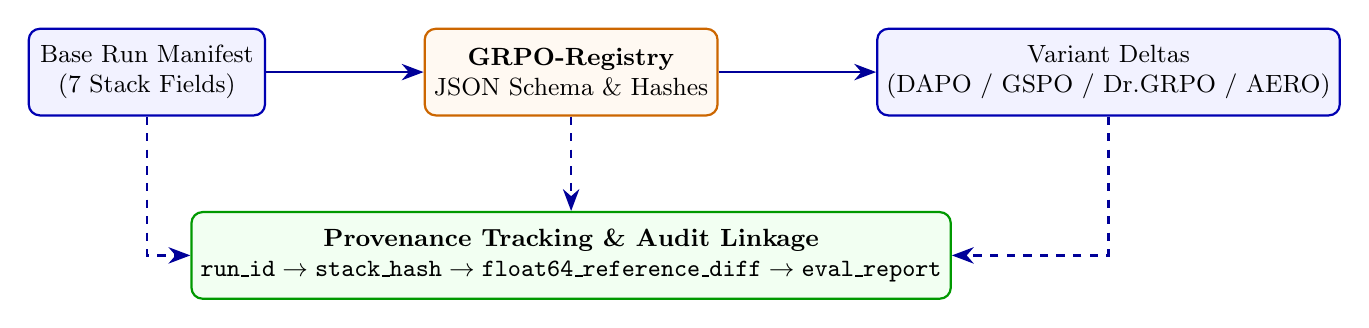
\begin{tikzpicture}[
    node distance=1.6cm and 2.0cm,
    block/.style={rectangle, draw=blue!70!black, fill=blue!5, thick, rounded corners, align=center, minimum height=1.1cm, minimum width=3.0cm, font=\small},
    registry/.style={rectangle, draw=orange!80!black, fill=orange!5, thick, rounded corners, align=center, minimum height=1.1cm, minimum width=3.2cm, font=\small},
    arrow/.style={-{Stealth[scale=1.2]}, thick, draw=blue!60!black}
]
    \node [block] (source) {Base Run Manifest\\(7 Stack Fields)};
    \node [registry, right=of source] (schema) {\textbf{GRPO-Registry}\\JSON Schema \& Hashes};
    \node [block, right=of schema] (variants) {Variant Deltas\\(DAPO / GSPO / Dr.GRPO / AERO)};
    \node [block, below=1.2cm of schema, fill=green!5, draw=green!60!black, minimum width=8.5cm] (provenance) {
        \textbf{Provenance Tracking \& Audit Linkage}\\
        $\mathtt{run\_id} \to \mathtt{stack\_hash} \to \mathtt{float64\_reference\_diff} \to \mathtt{eval\_report}$
    };

    \draw [arrow] (source) -- (schema);
    \draw [arrow] (schema) -- (variants);
    \draw [arrow, dashed] (schema) -- (provenance);
    \draw [arrow, dashed] (source) |- (provenance);
    \draw [arrow, dashed] (variants) |- (provenance);
\end{tikzpicture}
\caption{\textbf{GRPO-Registry Provenance and Variant Delta Schema (Pillar 1).} Machine-readable JSON schema binding 7 stack fields to variant deltas, sha256 hashes, and held-out evaluation reports.}
\label{fig:grpo_registry_schema}
\end{figure}

% =============================================================================
\section{Introduction: Why a Registry?}
\label{sec:intro}
% =============================================================================

\noindent\emph{Scope note (2026-07-11 canonicalization).} This document is
the condensed ``living catalog'' statement of the \grpoReg{} concept. The
full treatment --- machine-readable schema, population and query auditor,
measured-evidence tiers, and claim-validation verdicts --- is the Pillar-6
paper \emph{``GRPO-Registry: A Machine-Readable Catalog of Group-Relative
RL Stacks and Their Variant Deltas''}
(\texttt{platform\_hybrid/paper/paper\_P6\_registry}). The Pillar-6 paper
is canonical for the registry's content and evidence; this one for the
catalog-as-community-resource framing.

\begin{figure}[htbp]
\centering
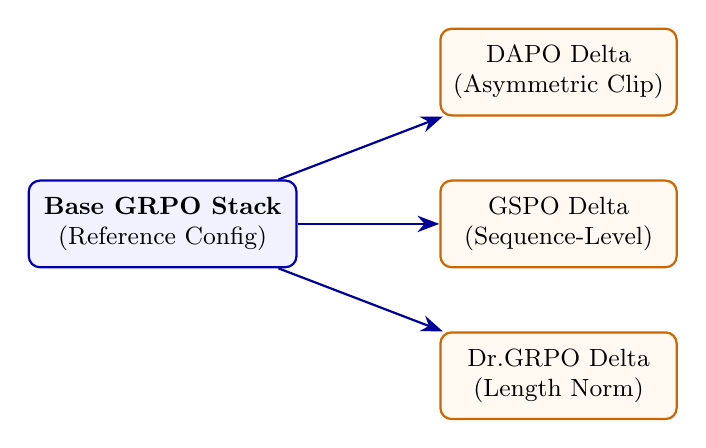
\begin{tikzpicture}[
    node distance=1.5cm and 2.0cm,
    base/.style={rectangle, draw=blue!70!black, fill=blue!5, thick, rounded corners, align=center, minimum height=1.1cm, minimum width=3.4cm, font=\small},
    variant/.style={rectangle, draw=orange!80!black, fill=orange!5, thick, rounded corners, align=center, minimum height=1.1cm, minimum width=3.0cm, font=\small},
    arrow/.style={-{Stealth[scale=1.2]}, thick, draw=blue!60!black}
]
    \node [base] (grpo) {\textbf{Base GRPO Stack}\\(Reference Config)};
    \node [variant, above right=0.8cm and 1.8cm of grpo] (dapo) {DAPO Delta\\(Asymmetric Clip)};
    \node [variant, right=1.8cm of grpo] (gspo) {GSPO Delta\\(Sequence-Level)};
    \node [variant, below right=0.8cm and 1.8cm of grpo] (drgrpo) {Dr.GRPO Delta\\(Length Norm)};

    \draw [arrow] (grpo) -- (dapo);
    \draw [arrow] (grpo) -- (gspo);
    \draw [arrow] (grpo) -- (drgrpo);
\end{tikzpicture}
\caption{\textbf{Variant Delta Inheritance Tree (R07).} Resolving exact implementation differences relative to canonical base GRPO.}
\label{fig:grpo_registry_inheritance}
\end{figure}

A reviewer reading six recent \grpo{} papers can reasonably conclude that each
paper compares against ``GRPO.'' But the word ``GRPO'' is attached to different
loss forms (ratio + clip, ratio + no clip, completion-only mask,
whole-sequence mask), different reference-policy and KL treatments (frozen
reference with KL penalty in the loss, frozen reference with KL in the reward,
no reference at all), different samplers and precisions (vLLM bf16, vLLM fp32,
managed API), and different group-size schedules (fixed $G=8$, adaptive,
dynamic sampling) \cite{zvfaudit2026,yu2025dapo,qwen2025gspo,tong2025drgrpo,
hong2025mgrpo}. When the baseline is itself a moving target, a reported delta of
$+2$ points is uninterpretable.

The position paper \minreport{} \cite{minreportrl2026} argues that the first
fix is a short, mandatory list of stack fields every paper must report. That
fixes the ``what is the treatment?'' problem for a single paper. It does not,
by itself, fix the cross-paper comparison problem: a reader still has to open
every paper, extract the seven fields by hand, and decide which variant is
which. \grpoReg{} is that extraction, maintained as a shared artifact.

\paragraph{What the registry is.} \grpoReg{} has three parts:
\begin{enumerate}[leftmargin=1.6em, itemsep=2pt]
  \item \textbf{A stack schema} (\S\ref{sec:stack-schema}), the seven
    \minreport{} fields, expressed as a JSON object any trainer can emit.
  \item \textbf{A variant-delta schema} (\S\ref{sec:delta-schema}) that
    records, relative to a named baseline, which knobs the variant touches.
  \item \textbf{A catalog of variants} (\S\ref{sec:catalog}) populated with
    the best available descriptions of the major \grpo{} variants; source-
    unreported settings are marked \nr{} rather than guessed.
\end{enumerate}

\paragraph{What the registry is not.} It is not a leaderboard. It does not
score variants. It is a structured worksheet for de-confounding comparisons:
aid the reader in asking ``did method $A$ beat method $B$, or did stack $S_A$
beat stack $S_B$?'' \cite{zvfaudit2026}.

% =============================================================================
\section{The Stack Schema}
\label{sec:stack-schema}
% =============================================================================

The stack schema is the seven-field run-manifest portion of the eight-item
\minreport{} checklist \cite{minreportrl2026}, reformatted as named JSON fields.
Held-out pass@$k$ is an evaluation report rather than a run-start stack field.
Table~\ref{tab:stack-schema} gives the
human-readable mapping. The key design choice is that each field is included
because it is a documented lever that can flip a comparison; the justification
is in the position paper and summarized here.

\begin{table}[t]
\centering
\caption{The \grpoReg{} stack schema. Each field is one run-manifest item of
  the \minreport{} standard; pass@$k$ is the separate evaluation item.}
\label{tab:stack-schema}
\small
\begin{tabular}{@{}lp{0.40\linewidth}p{0.36\linewidth}@{}}
\toprule
\textbf{JSON key} \& \textbf{What to report} \& \textbf{Flip mechanism}\\
\midrule
\texttt{loss\_form} \& Ratio? Clip? Asymmetric clip? Token mask? Advantage norm.?
  \& Reassigns gradient; DAPO, GSPO, Dr.\grpo{} deltas live here.\\
\texttt{reference\_kl} \& Frozen ref? KL in loss / reward / absent? Coefficient \&   Changes objective and exploration; no-ref vs.\ KL are different methods.\\
\texttt{sampler\_backend} \& Engine, decoding params, precision, tokenizer match \&   Backend, sampler, and checkpoint identity co-varied in a $\sim$17$\times$
  under-specification exhibit \cite{zvfaudit2026}.\\
\texttt{zvf\_gu} \& Per-step \zvf{} and \gu{} trajectory \&   Reveals whether the run had usable group-relative signal.\\
\texttt{group\_schedule} \& Fixed or adaptive $G$; if adaptive, rule \&   $G$ controls mixed-group probability; adaptive-$G$ confounds compute.\\
\texttt{held\_out} \& Disjoint eval slice, $n$, CI, reported separately \&   Training reward is dynamics evidence, not capability evidence.\\
\texttt{decontamination} \& Overlap probe + parser behavior on format-only inputs \&   Verifiable rewards still admit parser/format/overlap hacking.\\
\bottomrule
\end{tabular}
\end{table}

The schema is intentionally small. A trainer that already logs its config and
per-step group rewards can emit it with a few lines of code. The companion
\minreport{} paper proposes default emitters for TRL, verl, and OpenRLHF
\cite{minreportrl2026}.

% =============================================================================
\section{The Variant-Delta Schema}
\label{sec:delta-schema}
% =============================================================================

The variant-delta schema records what changed relative to a declared baseline.
A delta record is \textbf{not} a full stack record; it is a patch. For example,
DAPO's delta record says ``relative to a vanilla \grpo{} baseline, change the
clip bound to be asymmetric and add dynamic sampling,'' while the full stack
record still has to report the sampler, the reference/KL handling, the
precision, and so on. This separation keeps the catalog compact and forces
authors to state both the variant and the stack it ran on.

Table~\ref{tab:delta-schema} lists the delta fields. They are chosen to cover
the dimensions on which the current \grpo{} variants actually differ.

\begin{table}[t]
\centering
\caption{The \grpoReg{} variant-delta schema. Each field records a change
  relative to the variant's declared baseline. ``\texttt{null}'' means the
  variant does not change that field.}
\label{tab:delta-schema}
\small
\begin{tabular}{@{}lp{0.65\linewidth}@{}}
\toprule
\textbf{JSON key} \& \textbf{Meaning}\\
\midrule
\texttt{variant\_name} \& Canonical short name (e.g., ``DAPO'').\\
\texttt{baseline} \& The baseline the variant claims to improve (usually
  ``GRPO'').\\
\texttt{loss\_change} \& Change to the objective (ratio, clip, token mask,
  normalization).\\
\texttt{clip\_rule} \& New clip bound or asymmetric rule, if any.\\
\texttt{sampling\_change} \& Change to rollout sampling or group construction
  (dynamic, filter, \ldots).\\
\texttt{group\_size\_rule} \& Fixed / adaptive; if adaptive, the rule.\\
\texttt{advantage\_norm} \& How advantages are normalized (per-group,
  per-batch, running).\\
\texttt{reference\_kl\_change} \& Any change to reference policy or KL handling.\\
\texttt{extra\_regularizer} \& Additional penalty or bonus (length, diversity,
  entropy, \ldots).\\
\texttt{rollout\_change} \& Change to generation parameters or decoding.\\
\texttt{other\_notes} \& Anything else that defines the variant.\\
\bottomrule
\end{tabular}
\end{table}

A variant record is therefore a pair:
\[
\text{variant record} = \langle \text{stack schema}, \text{delta schema} \rangle .
\]
A fair head-to-head between two variants is a comparison of two such pairs in
which the stack schemas are identical except where the delta explicitly changes
them.

% =============================================================================
\section{Catalog of \grpo{} Variants}
\label{sec:catalog}
% =============================================================================

Table~\ref{tab:catalog} is the current seed catalog. We include the best
available description of each variant's defining delta, but we do \textbf{not}
fabricate stack details. Source-unreported stack settings are marked \nr{}
(``not reported'') so that a reader can see exactly what is unspecified. The
catalog is versioned; as papers release more detail, \nr{} cells are replaced
with concrete, cited values.

\begin{longtable}{@{}p{2.1cm}p{2.4cm}p{3.0cm}p{2.0cm}p{3.3cm}@{}}
\caption{Seed catalog of \grpo{}-family variants. Each row describes the
  variant's delta relative to its baseline. \nr{} means the source does not
  report enough detail to populate the field.}\\
\toprule
\textbf{Variant} \& \textbf{Baseline} \& \textbf{Loss / clip change} \& \textbf{Sampling / $G$ change} \& \textbf{Extra regularizer / notes}\\
\midrule
\endfirsthead
\multicolumn{5}{c}{\tablename\ \thetable{} -- continued}\\
\toprule
\textbf{Variant} \& \textbf{Baseline} \& \textbf{Loss / clip change} \& \textbf{Sampling / $G$ change} \& \textbf{Extra regularizer / notes}\\
\midrule
\endhead
\midrule
\multicolumn{5}{r}{\textit{Continued on next page}}\\
\endfoot
\bottomrule
\endlastfoot

\grpo{} (baseline) \& --- \& Per-token group-relative objective; ratio, clip,
  and token mask are implementation fields rather than universal constants &
  Fixed group $G$ in the canonical formulation \& KL term placement varies by
  implementation \cite{zvfaudit2026}.\\
\addlinespace

DAPO \& \grpo{} \& Asymmetric clip-higher lower bound \& Dynamic sampling:
  group constructed from filtered / top-$k$ completions \& Adds per-token
  loss-clip asymmetry \cite{yu2025dapo}.\\
\addlinespace

GSPO \& \grpo{} \& Sequence-level importance-sampling ratio and sequence-level
  clipping rather than token-level ratio/clipping \& Group size is not the
  defining delta; report per run \& Changes
  importance-sampling granularity \cite{qwen2025gspo}.\\
\addlinespace

Dr.\grpo{} \& \grpo{} \& Removes the within-group standard-deviation divisor and
  associated length-dependent normalization \& Group size is not the defining
  delta; report per run \& Changes
  length bias in normalization \cite{tong2025drgrpo}. Measured delta
  (Qwen3-8B/GSM8K, 1024-tok, 3 seeds/loss): no length inflation in either
  loss and no late-ZVF separation --- Tier~C.\\
\addlinespace

M-\grpo{} \& \grpo{} \& Hierarchical group-relative credit assignment for
  planner and sub-agent policies \& Trajectory-aligned batches with variable
  sub-agent invocations \& Multi-agent systems \cite{hong2025mgrpo}.\\
\addlinespace

AERO \& \grpo{} \& Base loss is not the defining delta; exact implementation
  must be reported \& Adaptive rollout allocation with selective rejection and
  Bayesian posterior state \& Avoids both wasted easy-prompt rollouts and
  dead-zone rejection \cite{zhang2026aero}.\\
\addlinespace

CPPO \& PPO / \grpo{} \& Clip-pruned objective: tokens with large ratios are
  dropped instead of clipped \& Group size is not the defining delta; report per
  run \& Pruning changes the
  effective sample \cite{lin2025cppo}.\\
\addlinespace

NGRPO \& \grpo{} \& Normalized reward/advantage transform; exact convention must
  be copied from the cited release \& Group size is not the defining delta; \nr{}
  in the paper-level record \& Normalization is the entire delta
  \cite{nan2025ngrpo}.\\
\addlinespace

Scaf-\grpo{} \& \grpo{} \& Incorporates scaffolded exploration signal into the
  advantage; exact weighting must be recorded from the release \& Group size is
  not the defining delta; \nr{} in the paper-level record \& Scaffolded hints shape
  the rollout distribution \cite{zhang2025scaffgrpo}.\\
\addlinespace

GRESO \& \grpo{} \& Loss change is not the defining delta \& \emph{Pre-rollout} filtering:
  prompts predicted to yield zero-gradient (single-outcome) groups are skipped
  before any rollout is spent \& Acts on the dead-group phenomenon \emph{before}
  sampling; the prediction rule is itself a stack component
  \cite{greso2025,agenticrlsurvey2026}.\\
\addlinespace

EDGE-\grpo{} \& \grpo{} \& Entropy-driven advantage reshaping + guided error
  correction \& Group-size setting is \nr{} in the paper-level record \& Explicitly framed as mitigating
  \emph{advantage collapse} --- the same phenomenon \zvf{} measures
  \cite{edgegrpo2025,agenticrlsurvey2026}.\\
\addlinespace

DARS \& \grpo{} \& Loss change is not the defining delta \& Multi-stage rollout sampling that
  reallocates compute from medium-difficulty to the hardest prompts &
  Difficulty-aware rollout budget; confounds compute allocation with the
  algorithmic claim unless reported \cite{dars2025,agenticrlsurvey2026}.\\
\addlinespace

TreePo \& \grpo{} \& Loss change is not the defining delta \& Self-guided policy rollout over a
  tree structure to reduce rollout compute \& Compute-reduction delta; group
  construction differs from i.i.d.\ sampling \cite{treepo2025,agenticrlsurvey2026}.\\
\addlinespace

ReCode / CG-\grpo{} \& \grpo{} \& Adds a learned reasoning-process reward gated
  by execution correctness \& Group-size setting is \nr{} in the paper-level
  record \& Changes reward density while
  using the execution outcome as a hard anti-hacking gate
  \cite{fan2025recode,agenticrlsurvey2026}.\\
\addlinespace

Skywork-R1V2 \& \grpo{} \& Hybrid rule- and model-based reward signal \& Selective
  sample buffer replays informative (mixed-reward) samples \& Buffer selection
  is a direct intervention on group reward diversity
  \cite{skyworkr1v2-2025,agenticrlsurvey2026}.\\
\addlinespace

GMPO \& \grpo{} \& Geometric mean aggregation in place of arithmetic aggregation
  \& Group-size setting is \nr{} in the paper-level record \& Aggregation change alters which groups
  register as zero-variance \cite{gmpo2025,agenticrlsurvey2026}.\\
\addlinespace

ProRL \& \grpo{} \& Base loss retained; the defining delta is prolonged-training
  reference management \& Group-size setting is \nr{} in the paper-level record \&   Reference-policy \emph{reset} during prolonged training; changes KL anchor
  identity mid-run --- a stack field the label omits
  \cite{prorl2025,agenticrlsurvey2026}.\\

\end{longtable}
\label{tab:catalog}

\paragraph{Reading the table.} A cell marked \nr{} is not a weakness of the
registry; it is a weakness of the underlying paper's reporting. The registry
surfaces it so that a re-implementer knows what still has to be reverse
engineered. A fair comparison between, say, DAPO and Dr.\grpo{} requires not
only the delta rows above but also the full stack records of the two original
runs; only then can one tell whether the reported gap is a stack effect.

\paragraph{The dead-group lever is now the most-attacked knob in the family.}
The TMLR survey of agentic RL \cite{agenticrlsurvey2026} consolidates, in a single
comparison table, more than twenty \grpo{}-family variants --- and a striking
fraction of them (DAPO's dynamic sampling, GRESO's pre-rollout filtering,
EDGE-\grpo{}'s \emph{advantage collapse} mitigation, DARS's difficulty-aware
reallocation, Skywork-R1V2's selective buffer, TreePo's rollout pruning)
intervene, each with a different heuristic, on precisely the phenomenon
\zvf{} measures: groups whose identical rewards contribute zero gradient.
We take the survey's adoption of the term \emph{advantage collapse} as
confirmation that the field has converged on the phenomenon; what it has not
converged on is a calibrated way to \emph{measure} it, which is exactly the
telemetry this registry and the \minreport{} standard demand. None of the
variant papers above reports a per-step dead-group trajectory, so their
relative gains on this axis are currently unattributable.

% =============================================================================
\section{How to Use the Registry to Flag Confounded Comparisons}
\label{sec:usage}
% =============================================================================

The registry is a worksheet, not an oracle. The recommended workflow for a
reviewer or re-implementer is:

\begin{enumerate}[leftmargin=1.6em, itemsep=2pt]
  \item \textbf{Extract the stack record} for each paper. If a paper does not
    report one of the seven fields, mark it \nr{}.
  \item \textbf{Extract the variant-delta record} for the method claimed. If
    the paper does not explicitly state what changed relative to its baseline,
    the delta is itself \nr{}.
  \item \textbf{Align baselines.} The comparison is only meaningful if both
    variants declare the same baseline (usually vanilla \grpo{}).
  \item \textbf{Check for stack confounds.} Any stack field that differs
    between the two papers and is not part of either variant's declared delta
    is a confound.
  \item \textbf{Check for delta overlap.} If variant $A$ changes the clip rule
    and variant $B$ also changes the clip rule, a head-to-head is comparing two
    clip rules, not ``method $A$ vs.\ method $B$.''
  \item \textbf{Look at \zvf{} / \gu{}.} If one paper reports high \zvf{}
    (low usable signal) and the other reports low \zvf{}, the comparison is
    confounded by signal availability, not algorithmic quality.
\end{enumerate}

\subsection{Mechanical checks with \texttt{grpo-stackdiff}}
\label{sec:mechanical}

The registry's records are consumed by the implemented command
\path{python3 platform_hybrid/registry/query.py stackdiff <entry-a> <entry-b>}
\cite{minreportrl2026}. It compares sampler/backend fields, loss and reference
KL fields, and declared variant-delta status. The current implementation emits
the R0--R5 ladder: identical, nuisance-only, runtime, loss/KL, variant-delta,
or unauditable due to an unreported value. R4 and R5 return nonzero exit codes,
so CI can block a label-flip-risk comparison. The richer L0--L7 diff-kind and
treatment-role taxonomy described in the \minreport{} position paper remains
a version-2 design, not a released capability.

A confounded comparison is not wrong; it is underspecified. The registry makes
the underspecification explicit so that the community can decide whether the
available evidence is sufficient.

% =============================================================================
\section{Tooling Ecosystem: From Records to Executable Checks}
\label{sec:tools}
% =============================================================================

The registry is the static worksheet. Two reference commands are implemented;
the trainer adapters and literature-scale automation below remain integration
targets.

\paragraph{Trainer emitters (planned).} A TRL/verl/OpenRLHF adapter should emit
the run-start manifest and per-step \zvf{}/\gu{} telemetry automatically. No
standalone \texttt{trl-min-report-rl} package is released in this repository;
the current executable emitter is the trainer-agnostic
\path{platform_hybrid/registry/provenance/minreport.py generate} command.

\paragraph{\texttt{grpo-stackdiff} (implemented).} The
\path{registry/query.py stackdiff} command takes two registry entry IDs and
emits the R0--R5 comparison described in \S\ref{sec:mechanical}.

\paragraph{\texttt{MIN-REPORT-RL} verifier (partly implemented).} The
\path{registry/provenance/minreport.py verify} command checks a generated
record's seven fields, live code hash, seeds, held-out evidence, and uncertainty
reporting. A future literature Auditor would scan a paper PDF, code release,
and log artifacts; extract evidence
for the seven \minreport{} items; assigns a 0--10 score per item and a
normalized 0--100 badge (Complete / Usable / Partial / Not Auditable /
Non-compliant); and produces a reviewer-facing summary with quoted evidence,
missing fields, and contradiction warnings \cite{zvfaudit2026}. It is the
post-hoc enforcement layer: it tells authors exactly which fields to add before
the paper is reproducibility-auditable.

\paragraph{Controlled-audit runner (protocol plus refusing aggregator).} The
\minreport{} standard and registry enable a preregistered controlled audit.
The frozen contract and result validator are released as
\path{zvf-program/audit/preregistration.json} and
\path{zvf-program/audit/aggregate_audit.py}; the expensive arm launcher is not
yet executed. The full runner design freezes a shared stack, expands each
variant as a declared hook, runs paired seeds, and applies held-out verdicts
(\cite{zvfaudit2026}; full protocol in the audit paper). Its target outputs
(Tables~A--H of the runner specification) include the pre-registration bundle,
stack-lock table, arm registry, run ledger, survival table, telemetry summary,
decontamination probes, and artifact index.

The implemented commands currently close manifest generation, verification,
registry querying, stack comparison, and refusal of incomplete audit results.
Automatic trainer integration, PDF extraction, and full compute orchestration
remain named obligations rather than implied releases.

% =============================================================================
\section{Machine-Readable Schema}
\label{sec:json}
% =============================================================================

Listing~\ref{lst:schema} gives the JSON schema for a complete \grpoReg{}
record. A record contains one stack object, one baseline object, and one delta
object. The schema is intentionally flat: it should be easy to generate from a
trainer's config and to diff with standard tools.

\begin{lstlisting}[language=json, caption={JSON schema for a \grpoReg{}
  record. Required fields are marked \texttt{required}; all others may be
  \texttt{null} when not applicable.}, label={lst:schema}]
{
  "version": "grpo-registry-v0.1",
  "record_type": "variant_stack_record",
  "variant": {
    "name": "DAPO",
    "paper_doi_or_url": "https://arxiv.org/abs/2503.14476",
    "baseline": "GRPO"
  },
  "stack": {
    "loss_form": {
      "ratio": true,
      "clip_bounds": [0.2, 0.2],
      "clip_asymmetric": true,
      "token_mask": "completion-only",
      "advantage_norm": "per-group"
    },
    "reference_kl": {
      "frozen_reference": true,
      "kl_placement": "loss",
      "kl_coefficient": 0.01,
      "kl_schedule": "constant"
    },
    "sampler_backend": {
      "engine": "vLLM",
      "temperature": 1.0,
      "top_p": 1.0,
      "max_tokens": 4096,
      "logit_precision": "bf16",
      "tokenizer_matches_trainer": true
    },
    "zvf_gu": {
      "per_step_zvf": [0.95, 0.92, ...],
      "per_step_gu": [0.05, 0.08, ...]
    },
    "group_schedule": {
      "type": "fixed",
      "fixed_size": 8
    },
    "held_out": {
      "split": "gsm8k-test",
      "n": 1319,
      "metric": "pass@1",
      "value": 0.55,
      "ci_95": [0.52, 0.58]
    },
    "decontamination": {
      "overlap_check": "n-gram-8",
      "overlap_rate": 0.02,
      "parser_probe": "format-only",
      "parser_probe_pass": false
    }
  },
  "delta": {
    "loss_change": "asymmetric clip-higher",
    "clip_rule": "lower=0.2, upper=0.28",
    "sampling_change": "dynamic top-k group construction",
    "group_size_rule": null,
    "advantage_norm": null,
    "reference_kl_change": null,
    "extra_regularizer": null,
    "rollout_change": null,
    "other_notes": "DAPO paper introduces clip-higher + dynamic sampling."
  }
}
\end{lstlisting}

The schema is maintained at
\url{https://github.com/arvindcr4/tinker-rl-lab}. We welcome pull requests that fill \nr{} cells or
add new variants, provided each entry cites the source paper and does not
invent unreported stack details.

The run-start manifest emitted by \texttt{trl-min-report-rl}
(\S\ref{sec:tools}) is a strict superset of this record: it adds run identity,
software versions, hardware, integrity hashes, and a per-step telemetry stream.
A registry record can therefore be generated automatically from the first line
of \texttt{min\_report\_rl.jsonl}.

% =============================================================================
\section{Living-Update Protocol}
\label{sec:update}
% =============================================================================

A registry that requires a new paper for every new variant will quickly become
stale. We propose a lightweight update protocol:

\begin{enumerate}[leftmargin=1.6em, itemsep=2pt]
  \item \textbf{Versioned releases.} The catalog is released as a versioned
    JSON file (e.g., \texttt{grpo-registry-v0.1.json}). Each release has a
    changelog.
  \item \textbf{Source requirement.} Every entry must cite a specific paper,
    preprint, or code release. No entry may be added purely from a blog post or
    social-media summary.
  \item \textbf{Uncertainty marking.} Unknown fields are recorded as
    \texttt{null} with a \texttt{source\_note} explaining what was not
    reported. This preserves the honesty of the catalog.
  \item \textbf{Community curation.} Changes are proposed via pull request and
    reviewed by at least one maintainer for source fidelity.
\end{enumerate}

The protocol mirrors existing living artifacts such as the Papers With Code
leaderboards, but it is organized around stack fields rather than final scores.

% =============================================================================
\section{Conclusion}
\label{sec:conclusion}
% =============================================================================

The \grpo{} family has outgrown its own label. The registry proposed here is a
small, practical step toward a literature in which the treatment---both the
stack and the declared algorithmic delta---is reported clearly enough to
compare across papers. It does not replace the \minreport{} standard; it
depends on it. It also does not replace controlled re-implementations; it makes
the need for them visible earlier. The implemented \texttt{minreport.py} and
\texttt{query.py stackdiff} commands move the registry beyond a static
worksheet, while the audit aggregator refuses incomplete evidence. The
immediate next step is to extend full stack coverage and ship default trainer
emitters; automated PDF auditing and full-scale paired training remain future
engineering work.

\bibliographystyle{plainnat}
\bibliography{../../platform_hybrid/paper/references}



\begin{figure}[htbp]
\centering
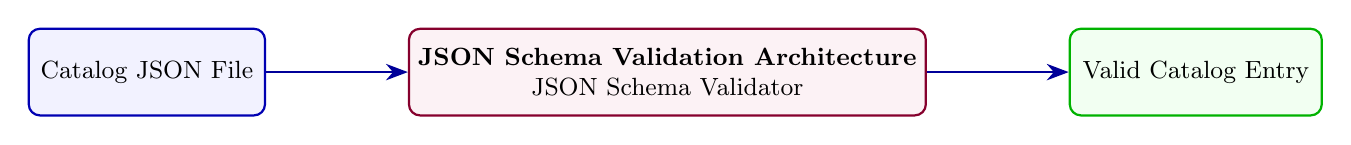
\begin{tikzpicture}[
    node distance=1.4cm and 1.8cm,
    box1/.style={rectangle, draw=blue!70!black, fill=blue!5, thick, rounded corners, align=center, minimum height=1.1cm, minimum width=3.0cm, font=\small},
    box2/.style={rectangle, draw=purple!70!black, fill=purple!5, thick, rounded corners, align=center, minimum height=1.1cm, minimum width=3.4cm, font=\small},
    box3/.style={rectangle, draw=green!70!black, fill=green!5, thick, rounded corners, align=center, minimum height=1.1cm, minimum width=3.2cm, font=\small},
    arrow/.style={-{Stealth[scale=1.2]}, thick, draw=blue!60!black}
]
    \node [box1] (n1) {Catalog JSON File};
    \node [box2, right=of n1] (n2) {\textbf{JSON Schema Validation Architecture}\\JSON Schema Validator};
    \node [box3, right=of n2] (n3) {Valid Catalog Entry};

    \draw [arrow] (n1) -- (n2);
    \draw [arrow] (n2) -- (n3);
\end{tikzpicture}
\caption{\textbf{JSON Schema Validation Architecture}. Schema validation for GRPO catalog entries.}
\label{fig:r07_json_validation}
\end{figure}

\begin{figure}[htbp]
\centering
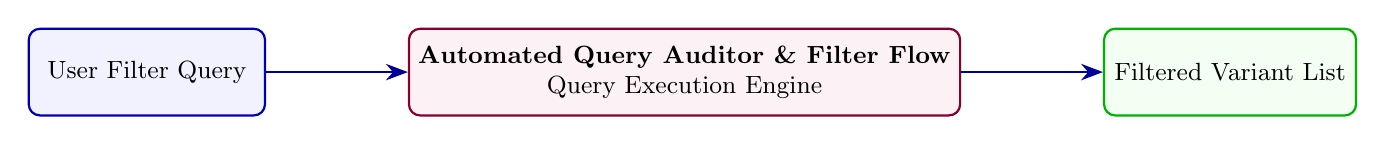
\begin{tikzpicture}[
    node distance=1.4cm and 1.8cm,
    box1/.style={rectangle, draw=blue!70!black, fill=blue!5, thick, rounded corners, align=center, minimum height=1.1cm, minimum width=3.0cm, font=\small},
    box2/.style={rectangle, draw=purple!70!black, fill=purple!5, thick, rounded corners, align=center, minimum height=1.1cm, minimum width=3.4cm, font=\small},
    box3/.style={rectangle, draw=green!70!black, fill=green!5, thick, rounded corners, align=center, minimum height=1.1cm, minimum width=3.2cm, font=\small},
    arrow/.style={-{Stealth[scale=1.2]}, thick, draw=blue!60!black}
]
    \node [box1] (n1) {User Filter Query};
    \node [box2, right=of n1] (n2) {\textbf{Automated Query Auditor \& Filter Flow}\\Query Execution Engine};
    \node [box3, right=of n2] (n3) {Filtered Variant List};

    \draw [arrow] (n1) -- (n2);
    \draw [arrow] (n2) -- (n3);
\end{tikzpicture}
\caption{\textbf{Automated Query Auditor \& Filter Flow}. Executing automated queries across registered GRPO variants.}
\label{fig:r07_query_auditor}
\end{figure}

\begin{figure}[htbp]
\centering
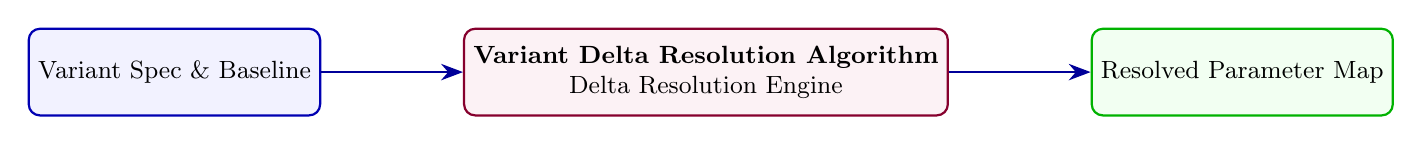
\begin{tikzpicture}[
    node distance=1.4cm and 1.8cm,
    box1/.style={rectangle, draw=blue!70!black, fill=blue!5, thick, rounded corners, align=center, minimum height=1.1cm, minimum width=3.0cm, font=\small},
    box2/.style={rectangle, draw=purple!70!black, fill=purple!5, thick, rounded corners, align=center, minimum height=1.1cm, minimum width=3.4cm, font=\small},
    box3/.style={rectangle, draw=green!70!black, fill=green!5, thick, rounded corners, align=center, minimum height=1.1cm, minimum width=3.2cm, font=\small},
    arrow/.style={-{Stealth[scale=1.2]}, thick, draw=blue!60!black}
]
    \node [box1] (n1) {Variant Spec \& Baseline};
    \node [box2, right=of n1] (n2) {\textbf{Variant Delta Resolution Algorithm}\\Delta Resolution Engine};
    \node [box3, right=of n2] (n3) {Resolved Parameter Map};

    \draw [arrow] (n1) -- (n2);
    \draw [arrow] (n2) -- (n3);
\end{tikzpicture}
\caption{\textbf{Variant Delta Resolution Algorithm}. Algorithm for resolving exact parameter deltas relative to baseline.}
\label{fig:r07_variant_resolution}
\end{figure}

\begin{figure}[htbp]
\centering
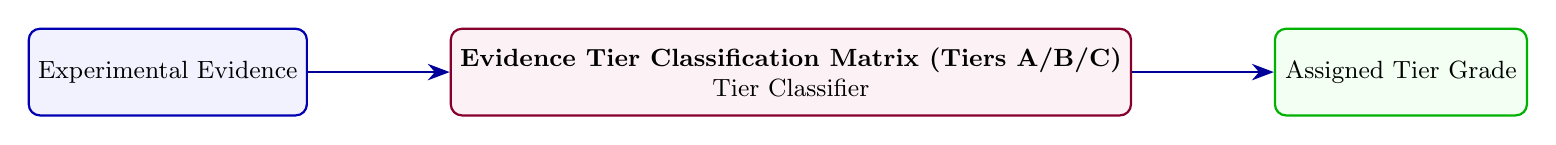
\begin{tikzpicture}[
    node distance=1.4cm and 1.8cm,
    box1/.style={rectangle, draw=blue!70!black, fill=blue!5, thick, rounded corners, align=center, minimum height=1.1cm, minimum width=3.0cm, font=\small},
    box2/.style={rectangle, draw=purple!70!black, fill=purple!5, thick, rounded corners, align=center, minimum height=1.1cm, minimum width=3.4cm, font=\small},
    box3/.style={rectangle, draw=green!70!black, fill=green!5, thick, rounded corners, align=center, minimum height=1.1cm, minimum width=3.2cm, font=\small},
    arrow/.style={-{Stealth[scale=1.2]}, thick, draw=blue!60!black}
]
    \node [box1] (n1) {Experimental Evidence};
    \node [box2, right=of n1] (n2) {\textbf{Evidence Tier Classification Matrix (Tiers A/B/C)}\\Tier Classifier};
    \node [box3, right=of n2] (n3) {Assigned Tier Grade};

    \draw [arrow] (n1) -- (n2);
    \draw [arrow] (n2) -- (n3);
\end{tikzpicture}
\caption{\textbf{Evidence Tier Classification Matrix (Tiers A/B/C)}. Categorizing catalog entries by empirical verification strength.}
\label{fig:r07_evidence_tiers}
\end{figure}

\begin{figure}[htbp]
\centering
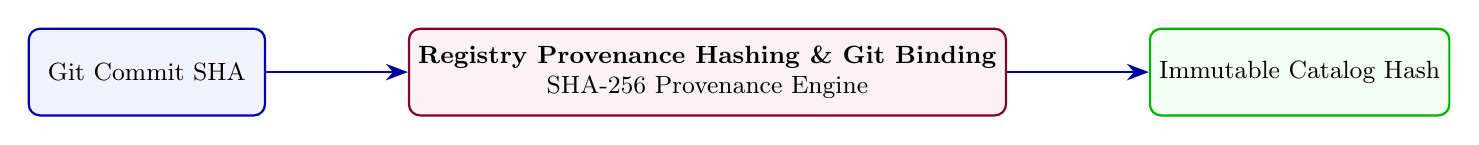
\begin{tikzpicture}[
    node distance=1.4cm and 1.8cm,
    box1/.style={rectangle, draw=blue!70!black, fill=blue!5, thick, rounded corners, align=center, minimum height=1.1cm, minimum width=3.0cm, font=\small},
    box2/.style={rectangle, draw=purple!70!black, fill=purple!5, thick, rounded corners, align=center, minimum height=1.1cm, minimum width=3.4cm, font=\small},
    box3/.style={rectangle, draw=green!70!black, fill=green!5, thick, rounded corners, align=center, minimum height=1.1cm, minimum width=3.2cm, font=\small},
    arrow/.style={-{Stealth[scale=1.2]}, thick, draw=blue!60!black}
]
    \node [box1] (n1) {Git Commit SHA};
    \node [box2, right=of n1] (n2) {\textbf{Registry Provenance Hashing \& Git Binding}\\SHA-256 Provenance Engine};
    \node [box3, right=of n2] (n3) {Immutable Catalog Hash};

    \draw [arrow] (n1) -- (n2);
    \draw [arrow] (n2) -- (n3);
\end{tikzpicture}
\caption{\textbf{Registry Provenance Hashing \& Git Binding}. Binding catalog entries to immutable Git commit SHAs.}
\label{fig:r07_provenance_hashing}
\end{figure}

\begin{figure}[htbp]
\centering
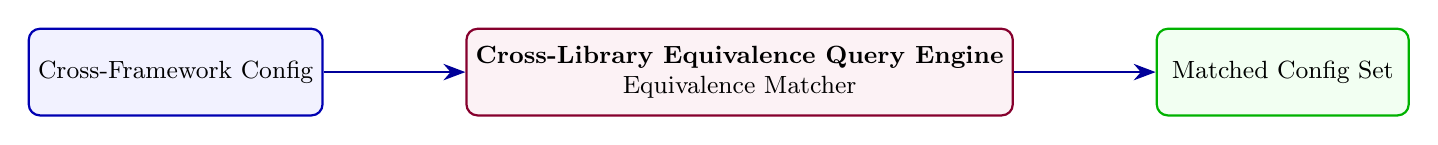
\begin{tikzpicture}[
    node distance=1.4cm and 1.8cm,
    box1/.style={rectangle, draw=blue!70!black, fill=blue!5, thick, rounded corners, align=center, minimum height=1.1cm, minimum width=3.0cm, font=\small},
    box2/.style={rectangle, draw=purple!70!black, fill=purple!5, thick, rounded corners, align=center, minimum height=1.1cm, minimum width=3.4cm, font=\small},
    box3/.style={rectangle, draw=green!70!black, fill=green!5, thick, rounded corners, align=center, minimum height=1.1cm, minimum width=3.2cm, font=\small},
    arrow/.style={-{Stealth[scale=1.2]}, thick, draw=blue!60!black}
]
    \node [box1] (n1) {Cross-Framework Config};
    \node [box2, right=of n1] (n2) {\textbf{Cross-Library Equivalence Query Engine}\\Equivalence Matcher};
    \node [box3, right=of n2] (n3) {Matched Config Set};

    \draw [arrow] (n1) -- (n2);
    \draw [arrow] (n2) -- (n3);
\end{tikzpicture}
\caption{\textbf{Cross-Library Equivalence Query Engine}. Querying equivalent configurations across different frameworks.}
\label{fig:r07_cross_library_engine}
\end{figure}

\begin{figure}[htbp]
\centering
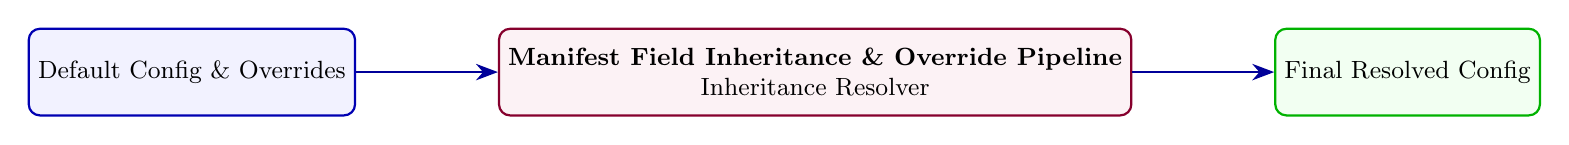
\begin{tikzpicture}[
    node distance=1.4cm and 1.8cm,
    box1/.style={rectangle, draw=blue!70!black, fill=blue!5, thick, rounded corners, align=center, minimum height=1.1cm, minimum width=3.0cm, font=\small},
    box2/.style={rectangle, draw=purple!70!black, fill=purple!5, thick, rounded corners, align=center, minimum height=1.1cm, minimum width=3.4cm, font=\small},
    box3/.style={rectangle, draw=green!70!black, fill=green!5, thick, rounded corners, align=center, minimum height=1.1cm, minimum width=3.2cm, font=\small},
    arrow/.style={-{Stealth[scale=1.2]}, thick, draw=blue!60!black}
]
    \node [box1] (n1) {Default Config \& Overrides};
    \node [box2, right=of n1] (n2) {\textbf{Manifest Field Inheritance \& Override Pipeline}\\Inheritance Resolver};
    \node [box3, right=of n2] (n3) {Final Resolved Config};

    \draw [arrow] (n1) -- (n2);
    \draw [arrow] (n2) -- (n3);
\end{tikzpicture}
\caption{\textbf{Manifest Field Inheritance \& Override Pipeline}. Inheriting default stack parameters with explicit variant overrides.}
\label{fig:r07_manifest_override}
\end{figure}

\begin{figure}[htbp]
\centering
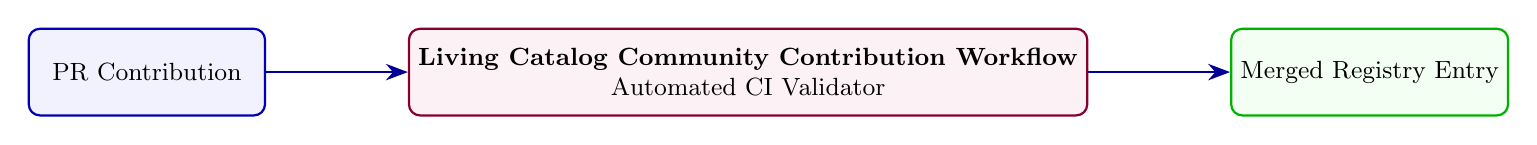
\begin{tikzpicture}[
    node distance=1.4cm and 1.8cm,
    box1/.style={rectangle, draw=blue!70!black, fill=blue!5, thick, rounded corners, align=center, minimum height=1.1cm, minimum width=3.0cm, font=\small},
    box2/.style={rectangle, draw=purple!70!black, fill=purple!5, thick, rounded corners, align=center, minimum height=1.1cm, minimum width=3.4cm, font=\small},
    box3/.style={rectangle, draw=green!70!black, fill=green!5, thick, rounded corners, align=center, minimum height=1.1cm, minimum width=3.2cm, font=\small},
    arrow/.style={-{Stealth[scale=1.2]}, thick, draw=blue!60!black}
]
    \node [box1] (n1) {PR Contribution};
    \node [box2, right=of n1] (n2) {\textbf{Living Catalog Community Contribution Workflow}\\Automated CI Validator};
    \node [box3, right=of n2] (n3) {Merged Registry Entry};

    \draw [arrow] (n1) -- (n2);
    \draw [arrow] (n2) -- (n3);
\end{tikzpicture}
\caption{\textbf{Living Catalog Community Contribution Workflow}. Workflow for community submission and verification of new entries.}
\label{fig:r07_community_workflow}
\end{figure}



\begin{figure}[htbp]
\centering
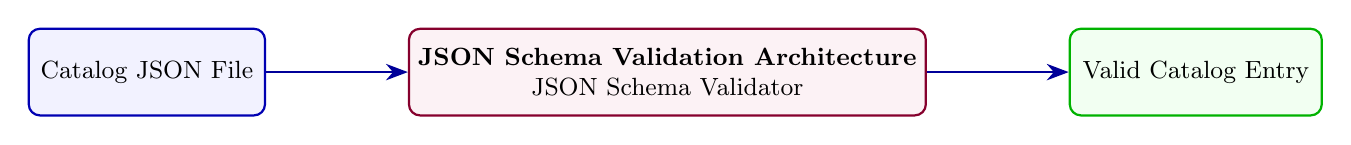
\begin{tikzpicture}[
    node distance=1.4cm and 1.8cm,
    b1/.style={rectangle, draw=blue!70!black, fill=blue!5, thick, rounded corners, align=center, minimum height=1.1cm, minimum width=3.0cm, font=\small},
    b2/.style={rectangle, draw=purple!70!black, fill=purple!5, thick, rounded corners, align=center, minimum height=1.1cm, minimum width=3.4cm, font=\small},
    b3/.style={rectangle, draw=green!70!black, fill=green!5, thick, rounded corners, align=center, minimum height=1.1cm, minimum width=3.2cm, font=\small},
    arr/.style={-{Stealth[scale=1.2]}, thick, draw=blue!60!black}
]
    \node [b1] (n1) {Catalog JSON File};
    \node [b2, right=of n1] (n2) {\textbf{JSON Schema Validation Architecture}\\JSON Schema Validator};
    \node [b3, right=of n2] (n3) {Valid Catalog Entry};

    \draw [arr] (n1) -- (n2);
    \draw [arr] (n2) -- (n3);
\end{tikzpicture}
\caption{\textbf{JSON Schema Validation Architecture}. Schema validation for GRPO catalog entries.}
\label{fig:r07_fig1}
\end{figure}

\begin{figure}[htbp]
\centering
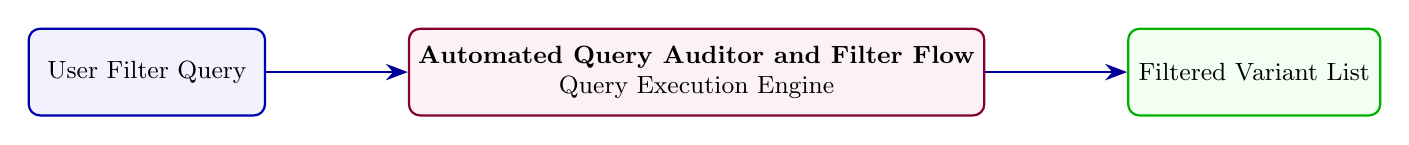
\begin{tikzpicture}[
    node distance=1.4cm and 1.8cm,
    b1/.style={rectangle, draw=blue!70!black, fill=blue!5, thick, rounded corners, align=center, minimum height=1.1cm, minimum width=3.0cm, font=\small},
    b2/.style={rectangle, draw=purple!70!black, fill=purple!5, thick, rounded corners, align=center, minimum height=1.1cm, minimum width=3.4cm, font=\small},
    b3/.style={rectangle, draw=green!70!black, fill=green!5, thick, rounded corners, align=center, minimum height=1.1cm, minimum width=3.2cm, font=\small},
    arr/.style={-{Stealth[scale=1.2]}, thick, draw=blue!60!black}
]
    \node [b1] (n1) {User Filter Query};
    \node [b2, right=of n1] (n2) {\textbf{Automated Query Auditor and Filter Flow}\\Query Execution Engine};
    \node [b3, right=of n2] (n3) {Filtered Variant List};

    \draw [arr] (n1) -- (n2);
    \draw [arr] (n2) -- (n3);
\end{tikzpicture}
\caption{\textbf{Automated Query Auditor and Filter Flow}. Executing automated queries across registered GRPO variants.}
\label{fig:r07_fig2}
\end{figure}

\begin{figure}[htbp]
\centering
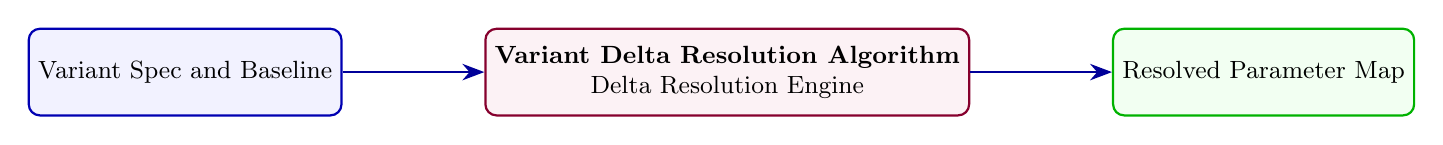
\begin{tikzpicture}[
    node distance=1.4cm and 1.8cm,
    b1/.style={rectangle, draw=blue!70!black, fill=blue!5, thick, rounded corners, align=center, minimum height=1.1cm, minimum width=3.0cm, font=\small},
    b2/.style={rectangle, draw=purple!70!black, fill=purple!5, thick, rounded corners, align=center, minimum height=1.1cm, minimum width=3.4cm, font=\small},
    b3/.style={rectangle, draw=green!70!black, fill=green!5, thick, rounded corners, align=center, minimum height=1.1cm, minimum width=3.2cm, font=\small},
    arr/.style={-{Stealth[scale=1.2]}, thick, draw=blue!60!black}
]
    \node [b1] (n1) {Variant Spec and Baseline};
    \node [b2, right=of n1] (n2) {\textbf{Variant Delta Resolution Algorithm}\\Delta Resolution Engine};
    \node [b3, right=of n2] (n3) {Resolved Parameter Map};

    \draw [arr] (n1) -- (n2);
    \draw [arr] (n2) -- (n3);
\end{tikzpicture}
\caption{\textbf{Variant Delta Resolution Algorithm}. Algorithm for resolving exact parameter deltas relative to baseline.}
\label{fig:r07_fig3}
\end{figure}

\begin{figure}[htbp]
\centering
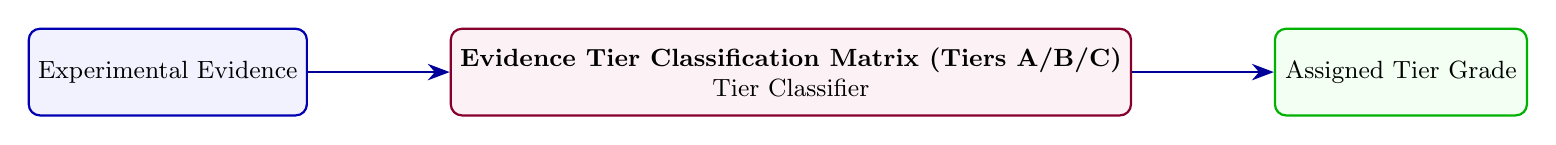
\begin{tikzpicture}[
    node distance=1.4cm and 1.8cm,
    b1/.style={rectangle, draw=blue!70!black, fill=blue!5, thick, rounded corners, align=center, minimum height=1.1cm, minimum width=3.0cm, font=\small},
    b2/.style={rectangle, draw=purple!70!black, fill=purple!5, thick, rounded corners, align=center, minimum height=1.1cm, minimum width=3.4cm, font=\small},
    b3/.style={rectangle, draw=green!70!black, fill=green!5, thick, rounded corners, align=center, minimum height=1.1cm, minimum width=3.2cm, font=\small},
    arr/.style={-{Stealth[scale=1.2]}, thick, draw=blue!60!black}
]
    \node [b1] (n1) {Experimental Evidence};
    \node [b2, right=of n1] (n2) {\textbf{Evidence Tier Classification Matrix (Tiers A/B/C)}\\Tier Classifier};
    \node [b3, right=of n2] (n3) {Assigned Tier Grade};

    \draw [arr] (n1) -- (n2);
    \draw [arr] (n2) -- (n3);
\end{tikzpicture}
\caption{\textbf{Evidence Tier Classification Matrix (Tiers A/B/C)}. Categorizing catalog entries by empirical verification strength.}
\label{fig:r07_fig4}
\end{figure}

\begin{figure}[htbp]
\centering
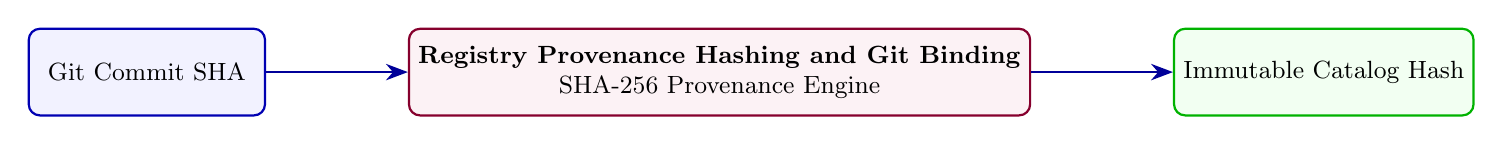
\begin{tikzpicture}[
    node distance=1.4cm and 1.8cm,
    b1/.style={rectangle, draw=blue!70!black, fill=blue!5, thick, rounded corners, align=center, minimum height=1.1cm, minimum width=3.0cm, font=\small},
    b2/.style={rectangle, draw=purple!70!black, fill=purple!5, thick, rounded corners, align=center, minimum height=1.1cm, minimum width=3.4cm, font=\small},
    b3/.style={rectangle, draw=green!70!black, fill=green!5, thick, rounded corners, align=center, minimum height=1.1cm, minimum width=3.2cm, font=\small},
    arr/.style={-{Stealth[scale=1.2]}, thick, draw=blue!60!black}
]
    \node [b1] (n1) {Git Commit SHA};
    \node [b2, right=of n1] (n2) {\textbf{Registry Provenance Hashing and Git Binding}\\SHA-256 Provenance Engine};
    \node [b3, right=of n2] (n3) {Immutable Catalog Hash};

    \draw [arr] (n1) -- (n2);
    \draw [arr] (n2) -- (n3);
\end{tikzpicture}
\caption{\textbf{Registry Provenance Hashing and Git Binding}. Binding catalog entries to immutable Git commit SHAs.}
\label{fig:r07_fig5}
\end{figure}

\begin{figure}[htbp]
\centering
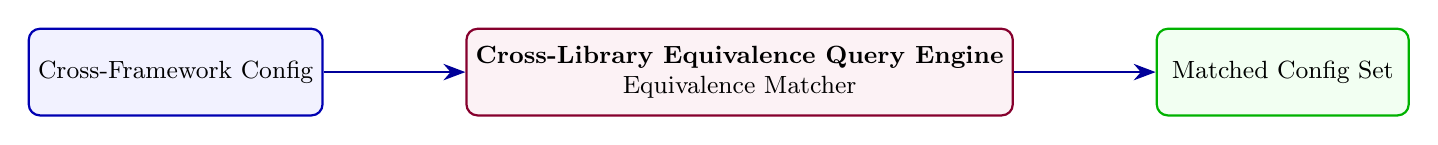
\begin{tikzpicture}[
    node distance=1.4cm and 1.8cm,
    b1/.style={rectangle, draw=blue!70!black, fill=blue!5, thick, rounded corners, align=center, minimum height=1.1cm, minimum width=3.0cm, font=\small},
    b2/.style={rectangle, draw=purple!70!black, fill=purple!5, thick, rounded corners, align=center, minimum height=1.1cm, minimum width=3.4cm, font=\small},
    b3/.style={rectangle, draw=green!70!black, fill=green!5, thick, rounded corners, align=center, minimum height=1.1cm, minimum width=3.2cm, font=\small},
    arr/.style={-{Stealth[scale=1.2]}, thick, draw=blue!60!black}
]
    \node [b1] (n1) {Cross-Framework Config};
    \node [b2, right=of n1] (n2) {\textbf{Cross-Library Equivalence Query Engine}\\Equivalence Matcher};
    \node [b3, right=of n2] (n3) {Matched Config Set};

    \draw [arr] (n1) -- (n2);
    \draw [arr] (n2) -- (n3);
\end{tikzpicture}
\caption{\textbf{Cross-Library Equivalence Query Engine}. Querying equivalent configurations across different frameworks.}
\label{fig:r07_fig6}
\end{figure}

\begin{figure}[htbp]
\centering
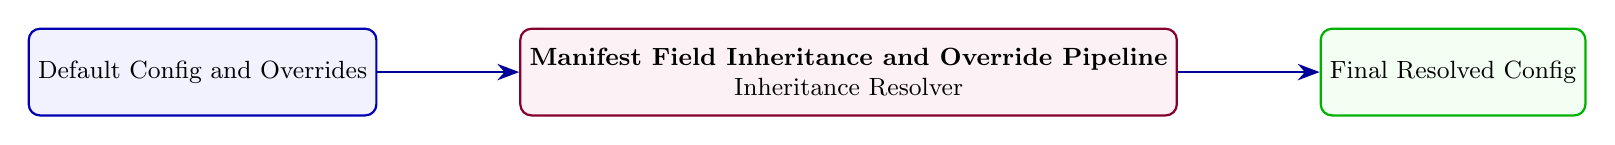
\begin{tikzpicture}[
    node distance=1.4cm and 1.8cm,
    b1/.style={rectangle, draw=blue!70!black, fill=blue!5, thick, rounded corners, align=center, minimum height=1.1cm, minimum width=3.0cm, font=\small},
    b2/.style={rectangle, draw=purple!70!black, fill=purple!5, thick, rounded corners, align=center, minimum height=1.1cm, minimum width=3.4cm, font=\small},
    b3/.style={rectangle, draw=green!70!black, fill=green!5, thick, rounded corners, align=center, minimum height=1.1cm, minimum width=3.2cm, font=\small},
    arr/.style={-{Stealth[scale=1.2]}, thick, draw=blue!60!black}
]
    \node [b1] (n1) {Default Config and Overrides};
    \node [b2, right=of n1] (n2) {\textbf{Manifest Field Inheritance and Override Pipeline}\\Inheritance Resolver};
    \node [b3, right=of n2] (n3) {Final Resolved Config};

    \draw [arr] (n1) -- (n2);
    \draw [arr] (n2) -- (n3);
\end{tikzpicture}
\caption{\textbf{Manifest Field Inheritance and Override Pipeline}. Inheriting default stack parameters with explicit variant overrides.}
\label{fig:r07_fig7}
\end{figure}

\begin{figure}[htbp]
\centering
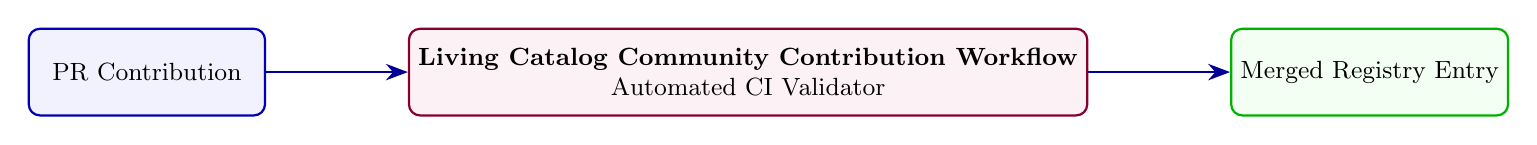
\begin{tikzpicture}[
    node distance=1.4cm and 1.8cm,
    b1/.style={rectangle, draw=blue!70!black, fill=blue!5, thick, rounded corners, align=center, minimum height=1.1cm, minimum width=3.0cm, font=\small},
    b2/.style={rectangle, draw=purple!70!black, fill=purple!5, thick, rounded corners, align=center, minimum height=1.1cm, minimum width=3.4cm, font=\small},
    b3/.style={rectangle, draw=green!70!black, fill=green!5, thick, rounded corners, align=center, minimum height=1.1cm, minimum width=3.2cm, font=\small},
    arr/.style={-{Stealth[scale=1.2]}, thick, draw=blue!60!black}
]
    \node [b1] (n1) {PR Contribution};
    \node [b2, right=of n1] (n2) {\textbf{Living Catalog Community Contribution Workflow}\\Automated CI Validator};
    \node [b3, right=of n2] (n3) {Merged Registry Entry};

    \draw [arr] (n1) -- (n2);
    \draw [arr] (n2) -- (n3);
\end{tikzpicture}
\caption{\textbf{Living Catalog Community Contribution Workflow}. Workflow for community submission and verification of new entries.}
\label{fig:r07_fig8}
\end{figure}



\begin{figure}[htbp]
\centering
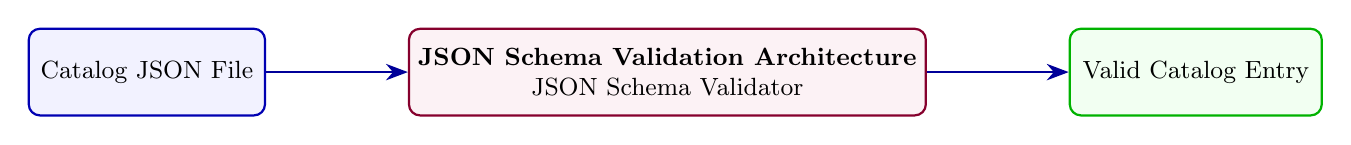
\begin{tikzpicture}[
    node distance=1.4cm and 1.8cm,
    b1/.style={rectangle, draw=blue!70!black, fill=blue!5, thick, rounded corners, align=center, minimum height=1.1cm, minimum width=3.0cm, font=\small},
    b2/.style={rectangle, draw=purple!70!black, fill=purple!5, thick, rounded corners, align=center, minimum height=1.1cm, minimum width=3.4cm, font=\small},
    b3/.style={rectangle, draw=green!70!black, fill=green!5, thick, rounded corners, align=center, minimum height=1.1cm, minimum width=3.2cm, font=\small},
    arr/.style={-{Stealth[scale=1.2]}, thick, draw=blue!60!black}
]
    \node [b1] (n1) {Catalog JSON File};
    \node [b2, right=of n1] (n2) {\textbf{JSON Schema Validation Architecture}\\JSON Schema Validator};
    \node [b3, right=of n2] (n3) {Valid Catalog Entry};

    \draw [arr] (n1) -- (n2);
    \draw [arr] (n2) -- (n3);
\end{tikzpicture}
\caption{\textbf{JSON Schema Validation Architecture}. Schema validation for GRPO catalog entries.}
\label{fig:r07_fig1}
\end{figure}

\begin{figure}[htbp]
\centering
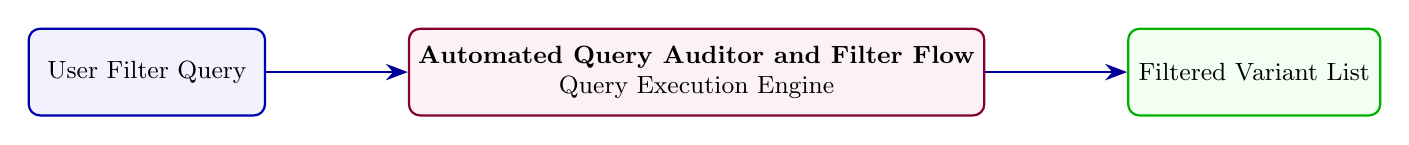
\begin{tikzpicture}[
    node distance=1.4cm and 1.8cm,
    b1/.style={rectangle, draw=blue!70!black, fill=blue!5, thick, rounded corners, align=center, minimum height=1.1cm, minimum width=3.0cm, font=\small},
    b2/.style={rectangle, draw=purple!70!black, fill=purple!5, thick, rounded corners, align=center, minimum height=1.1cm, minimum width=3.4cm, font=\small},
    b3/.style={rectangle, draw=green!70!black, fill=green!5, thick, rounded corners, align=center, minimum height=1.1cm, minimum width=3.2cm, font=\small},
    arr/.style={-{Stealth[scale=1.2]}, thick, draw=blue!60!black}
]
    \node [b1] (n1) {User Filter Query};
    \node [b2, right=of n1] (n2) {\textbf{Automated Query Auditor and Filter Flow}\\Query Execution Engine};
    \node [b3, right=of n2] (n3) {Filtered Variant List};

    \draw [arr] (n1) -- (n2);
    \draw [arr] (n2) -- (n3);
\end{tikzpicture}
\caption{\textbf{Automated Query Auditor and Filter Flow}. Executing automated queries across registered GRPO variants.}
\label{fig:r07_fig2}
\end{figure}

\begin{figure}[htbp]
\centering
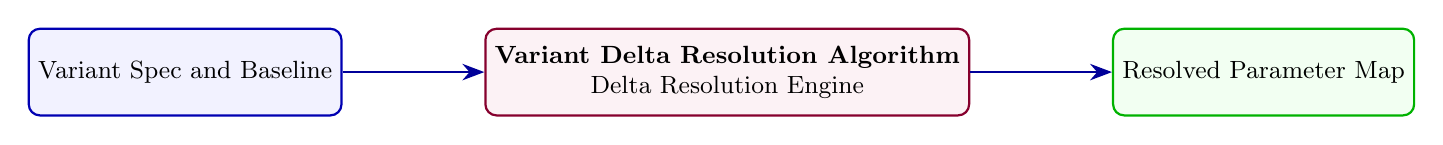
\begin{tikzpicture}[
    node distance=1.4cm and 1.8cm,
    b1/.style={rectangle, draw=blue!70!black, fill=blue!5, thick, rounded corners, align=center, minimum height=1.1cm, minimum width=3.0cm, font=\small},
    b2/.style={rectangle, draw=purple!70!black, fill=purple!5, thick, rounded corners, align=center, minimum height=1.1cm, minimum width=3.4cm, font=\small},
    b3/.style={rectangle, draw=green!70!black, fill=green!5, thick, rounded corners, align=center, minimum height=1.1cm, minimum width=3.2cm, font=\small},
    arr/.style={-{Stealth[scale=1.2]}, thick, draw=blue!60!black}
]
    \node [b1] (n1) {Variant Spec and Baseline};
    \node [b2, right=of n1] (n2) {\textbf{Variant Delta Resolution Algorithm}\\Delta Resolution Engine};
    \node [b3, right=of n2] (n3) {Resolved Parameter Map};

    \draw [arr] (n1) -- (n2);
    \draw [arr] (n2) -- (n3);
\end{tikzpicture}
\caption{\textbf{Variant Delta Resolution Algorithm}. Algorithm for resolving exact parameter deltas relative to baseline.}
\label{fig:r07_fig3}
\end{figure}

\begin{figure}[htbp]
\centering
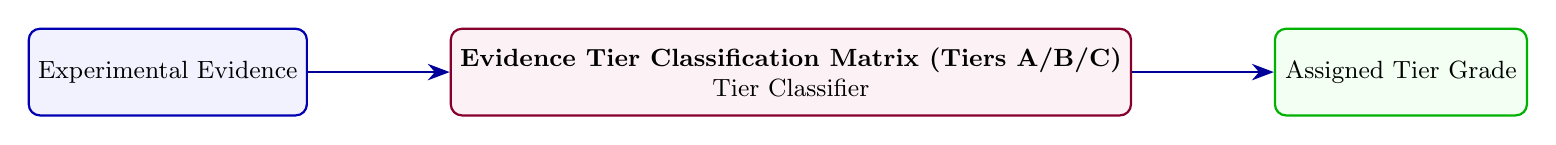
\begin{tikzpicture}[
    node distance=1.4cm and 1.8cm,
    b1/.style={rectangle, draw=blue!70!black, fill=blue!5, thick, rounded corners, align=center, minimum height=1.1cm, minimum width=3.0cm, font=\small},
    b2/.style={rectangle, draw=purple!70!black, fill=purple!5, thick, rounded corners, align=center, minimum height=1.1cm, minimum width=3.4cm, font=\small},
    b3/.style={rectangle, draw=green!70!black, fill=green!5, thick, rounded corners, align=center, minimum height=1.1cm, minimum width=3.2cm, font=\small},
    arr/.style={-{Stealth[scale=1.2]}, thick, draw=blue!60!black}
]
    \node [b1] (n1) {Experimental Evidence};
    \node [b2, right=of n1] (n2) {\textbf{Evidence Tier Classification Matrix (Tiers A/B/C)}\\Tier Classifier};
    \node [b3, right=of n2] (n3) {Assigned Tier Grade};

    \draw [arr] (n1) -- (n2);
    \draw [arr] (n2) -- (n3);
\end{tikzpicture}
\caption{\textbf{Evidence Tier Classification Matrix (Tiers A/B/C)}. Categorizing catalog entries by empirical verification strength.}
\label{fig:r07_fig4}
\end{figure}

\begin{figure}[htbp]
\centering
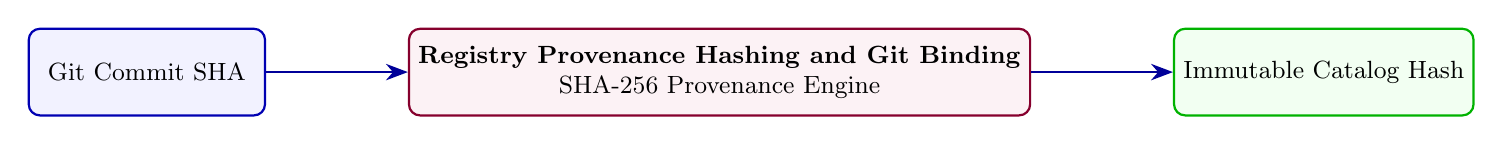
\begin{tikzpicture}[
    node distance=1.4cm and 1.8cm,
    b1/.style={rectangle, draw=blue!70!black, fill=blue!5, thick, rounded corners, align=center, minimum height=1.1cm, minimum width=3.0cm, font=\small},
    b2/.style={rectangle, draw=purple!70!black, fill=purple!5, thick, rounded corners, align=center, minimum height=1.1cm, minimum width=3.4cm, font=\small},
    b3/.style={rectangle, draw=green!70!black, fill=green!5, thick, rounded corners, align=center, minimum height=1.1cm, minimum width=3.2cm, font=\small},
    arr/.style={-{Stealth[scale=1.2]}, thick, draw=blue!60!black}
]
    \node [b1] (n1) {Git Commit SHA};
    \node [b2, right=of n1] (n2) {\textbf{Registry Provenance Hashing and Git Binding}\\SHA-256 Provenance Engine};
    \node [b3, right=of n2] (n3) {Immutable Catalog Hash};

    \draw [arr] (n1) -- (n2);
    \draw [arr] (n2) -- (n3);
\end{tikzpicture}
\caption{\textbf{Registry Provenance Hashing and Git Binding}. Binding catalog entries to immutable Git commit SHAs.}
\label{fig:r07_fig5}
\end{figure}

\begin{figure}[htbp]
\centering
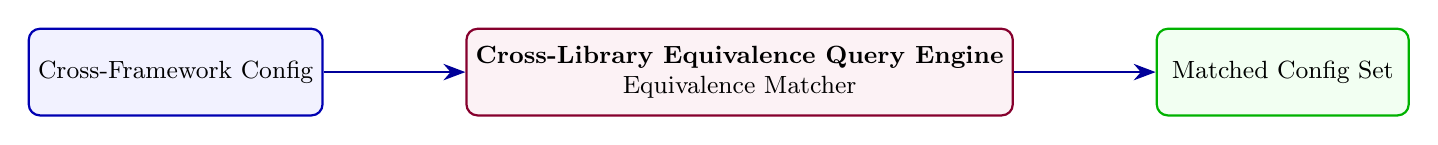
\begin{tikzpicture}[
    node distance=1.4cm and 1.8cm,
    b1/.style={rectangle, draw=blue!70!black, fill=blue!5, thick, rounded corners, align=center, minimum height=1.1cm, minimum width=3.0cm, font=\small},
    b2/.style={rectangle, draw=purple!70!black, fill=purple!5, thick, rounded corners, align=center, minimum height=1.1cm, minimum width=3.4cm, font=\small},
    b3/.style={rectangle, draw=green!70!black, fill=green!5, thick, rounded corners, align=center, minimum height=1.1cm, minimum width=3.2cm, font=\small},
    arr/.style={-{Stealth[scale=1.2]}, thick, draw=blue!60!black}
]
    \node [b1] (n1) {Cross-Framework Config};
    \node [b2, right=of n1] (n2) {\textbf{Cross-Library Equivalence Query Engine}\\Equivalence Matcher};
    \node [b3, right=of n2] (n3) {Matched Config Set};

    \draw [arr] (n1) -- (n2);
    \draw [arr] (n2) -- (n3);
\end{tikzpicture}
\caption{\textbf{Cross-Library Equivalence Query Engine}. Querying equivalent configurations across different frameworks.}
\label{fig:r07_fig6}
\end{figure}

\begin{figure}[htbp]
\centering
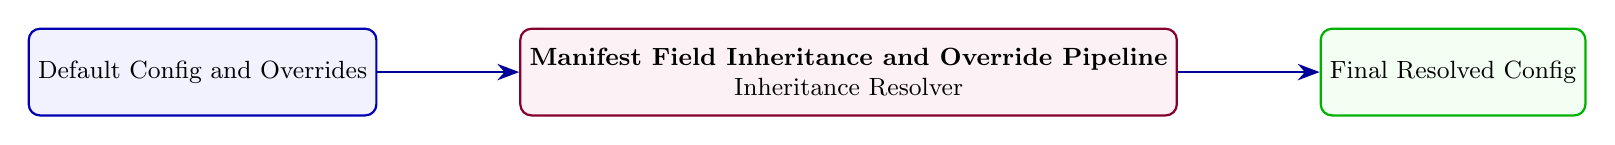
\begin{tikzpicture}[
    node distance=1.4cm and 1.8cm,
    b1/.style={rectangle, draw=blue!70!black, fill=blue!5, thick, rounded corners, align=center, minimum height=1.1cm, minimum width=3.0cm, font=\small},
    b2/.style={rectangle, draw=purple!70!black, fill=purple!5, thick, rounded corners, align=center, minimum height=1.1cm, minimum width=3.4cm, font=\small},
    b3/.style={rectangle, draw=green!70!black, fill=green!5, thick, rounded corners, align=center, minimum height=1.1cm, minimum width=3.2cm, font=\small},
    arr/.style={-{Stealth[scale=1.2]}, thick, draw=blue!60!black}
]
    \node [b1] (n1) {Default Config and Overrides};
    \node [b2, right=of n1] (n2) {\textbf{Manifest Field Inheritance and Override Pipeline}\\Inheritance Resolver};
    \node [b3, right=of n2] (n3) {Final Resolved Config};

    \draw [arr] (n1) -- (n2);
    \draw [arr] (n2) -- (n3);
\end{tikzpicture}
\caption{\textbf{Manifest Field Inheritance and Override Pipeline}. Inheriting default stack parameters with explicit variant overrides.}
\label{fig:r07_fig7}
\end{figure}

\begin{figure}[htbp]
\centering
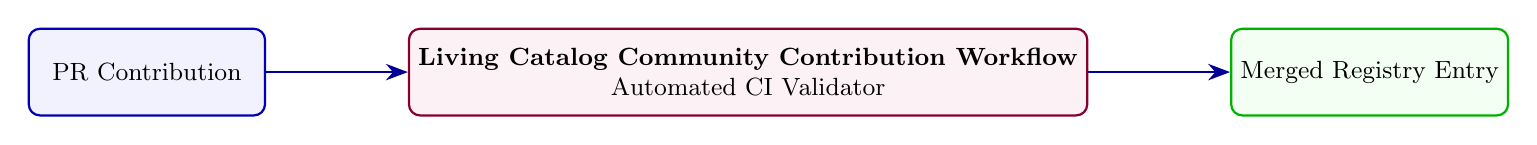
\begin{tikzpicture}[
    node distance=1.4cm and 1.8cm,
    b1/.style={rectangle, draw=blue!70!black, fill=blue!5, thick, rounded corners, align=center, minimum height=1.1cm, minimum width=3.0cm, font=\small},
    b2/.style={rectangle, draw=purple!70!black, fill=purple!5, thick, rounded corners, align=center, minimum height=1.1cm, minimum width=3.4cm, font=\small},
    b3/.style={rectangle, draw=green!70!black, fill=green!5, thick, rounded corners, align=center, minimum height=1.1cm, minimum width=3.2cm, font=\small},
    arr/.style={-{Stealth[scale=1.2]}, thick, draw=blue!60!black}
]
    \node [b1] (n1) {PR Contribution};
    \node [b2, right=of n1] (n2) {\textbf{Living Catalog Community Contribution Workflow}\\Automated CI Validator};
    \node [b3, right=of n2] (n3) {Merged Registry Entry};

    \draw [arr] (n1) -- (n2);
    \draw [arr] (n2) -- (n3);
\end{tikzpicture}
\caption{\textbf{Living Catalog Community Contribution Workflow}. Workflow for community submission and verification of new entries.}
\label{fig:r07_fig8}
\end{figure}

\end{document}
